\chapter{Retrosintesis dan Strategi Multitahap}\label{ch:b2:retrosynthesis}

Sebuah molekul digambar di papan, dan belum ada yang tahu cara membuatnya.
Mencoba reaksi-reaksi ke arah maju, dari apa pun yang ada di rak, tidak
membawa ke mana-mana: kemungkinannya terlalu banyak. Kimiawan bekerja ke
arah sebaliknya, dari target kembali ke rak, dengan memotong satu ikatan
demi satu ikatan di atas kertas, yang setiap potongannya membatalkan sebuah
reaksi yang diketahui berhasil, sampai potongan-potongannya berupa senyawa
yang dapat dibeli. Bab ini mengubah reaksi-reaksi dari bab-bab sebelumnya
menjadi penalaran mundur itu, lalu menanyakan bagaimana menilai jalur yang
dihasilkannya.

\begin{recall}
\Cref{ch:b2:alkene-redox} sampai \cref{ch:b2:wittig}: reaksi-reaksi yang
akan dibatalkan. Jilid Tahun 1: gugus pelindung dan asetal, pereaksi
Grignard dan pembalikan kepolaran, sintesis Williamson, kemoselektivitas,
oksidasi alkohol. Jilid sekolah: ekonomi atom.
\end{recall}

\section{Berpikir mundur}

\begin{definition}[Analisis retrosintetik]\label{def:b2:retrosynthesis:analysis}
Molekul yang akan dibuat disebut \emph{molekul target}\index{molekul target}. \emph{Analisis retrosintetik}
\index{analisis retrosintetik} bekerja dari target kembali ke bahan awal
yang tersedia, melalui tahap-tahap yang masing-masing merupakan kebalikan
sebuah reaksi yang dikenal; satu tahap retrosintetik ditulis dengan panah
ganda $\Rightarrow$, yang dibaca ``dibuat dari''.
\end{definition}

\begin{definition}[Pemutusan dan sinton]\label{def:b2:retrosynthesis:disconnection}
Yang disebut \emph{pemutusan}\index{pemutusan} adalah pemotongan khayal
sebuah ikatan target, kebalikan dari reaksi pembentuk ikatan. Memotong
ikatan secara heterolitik menghasilkan dua \emph{sinton}\index{sinton},
yaitu fragmen bermuatan yang diidealkan, yang satu donor (nukleofilik,
sering negatif), yang lain akseptor (elektrofilik, sering positif). Yang
disebut \emph{ekuivalen sintetik}\index{ekuivalen sintetik} adalah pereaksi
nyata yang berperilaku sebagai sinton: pereaksi Grignard untuk karbanion
\ce{R-}, aldehida untuk kation $\mathrm{R\overset{+}{C}H{-}OH}$.
\end{definition}

\begin{definition}[Interkonversi gugus fungsi]\label{def:b2:retrosynthesis:fgi}
Yang disebut \emph{interkonversi gugus fungsi}\index{interkonversi gugus fungsi}
(FGI) adalah tahap retrosintetik yang mengubah sebuah gugus fungsi tanpa
mengubah kerangka karbon: alkohol dari keton (melalui reduksi), rantai
alkana dari alkena (melalui hidrogenasi), amina dari amida.
\end{definition}

\begin{omfigure}
\begin{tikzpicture}[every node/.style={align=center}]
\node (T) at (0,0) {\setchemfig{atom sep=1.7em}\chemfig{Ph-CH(-[2]OH)-CH(-[6]CH_3)-CH_3}};
\node (A) at (-4.6,-2.6) {\ce{PhCHO}\\[1pt] + \ce{(CH3)2CHMgBr}};
\node (B) at (0,-2.6) {\ce{PhMgBr}\\[1pt] + \ce{(CH3)2CHCHO}};
\node (C) at (4.6,-2.6) {\setchemfig{atom sep=1.7em}\chemfig{Ph-C(=[2]O)-CH(-[6]CH_3)-CH_3}};
\node (D) at (4.6,-5.0) {\ce{C6H6}\\[1pt] + \ce{(CH3)2CHCOCl}};
\draw[omretro] (T.south west) -- node[above left, font=\small] {a} (A.north);
\draw[omretro] (T.south) -- node[right, font=\small] {b} (B.north);
\draw[omretro] (T.south east) -- node[above right, font=\small] {FGI} (C.north);
\draw[omretro] (C.south) -- node[right, font=\small] {c} (D.north);
\end{tikzpicture}
\par\vspace{6pt}

{\small Pohon retrosintetik untuk 2-metil-1-fenilpropan-1-ol. (a) dan (b):
kedua \omterm{def:b2:retrosynthesis:disconnection}{pemutusan} ikatan \ce{C-C} di sebelah karbon alkohol, masing-masing
menjadi aldehida dan pereaksi Grignard. FGI: alkohol dari keton, melalui
reduksi; (c) keton itu melalui \omterm{def:b2:aromatic-substitution:friedel-crafts}{asilasi Friedel--Crafts} benzena. Setiap
panah dibaca ``dibuat dari''.}
\end{omfigure}

Pohon itu memperlihatkan kebiasaan-kebiasaan metode ini. \omterm{def:b2:retrosynthesis:disconnection}{Pemutusan} dipilih
pada ikatan di sebelah gugus fungsi, karena di sanalah reaksi-reaksi
membentuk ikatan. Setiap potongan diperiksa dengan menuliskan \omterm{def:b2:retrosynthesis:disconnection}{sinton-sintonnya}
dan mencari pereaksi nyata untuknya. Dan jarang ada satu jawaban saja: pohon
itu bercabang, dan cabang-cabangnya dinilai di akhir
(\cref{sec:b2:retrosynthesis:judging}).

\begin{omfigure}
\begin{center}
\small
\renewcommand{\arraystretch}{1.25}
\begin{tabular}{lll}
\hline
\omterm{def:b2:retrosynthesis:disconnection}{Sinton} & Jenis & \omterm{def:b2:retrosynthesis:disconnection}{Ekuivalen sintetik} \\
\hline
\ce{R-} (alkil, aril) & donor & \ce{RMgBr}, \ce{RLi}, \ce{R2CuLi} (konjugat) \\
$\mathrm{^-CH_2COR}$ & donor & \omterm{def:b2:enolates-aldol:enolate}{enolat} \ce{CH3COR}, atau etil 3-oksobutanoat \\
$\mathrm{^-C{\equiv}N}$ & donor & \ce{NaCN} \\
$\mathrm{R\overset{+}{C}H{-}OH}$ & akseptor & aldehida \ce{RCHO} \\
$\mathrm{R\overset{+}{C}{=}O}$ & akseptor & \omterm{def:b2:acyl-substitution:derivative}{asil klorida} \ce{RCOCl}, ester \\
\ce{R+} (primer) & akseptor & halida \ce{RBr} (substitusi bimolekular) \\
$\mathrm{^+CH_2CH_2COR}$ & akseptor & enon \ce{CH2=CHCOR} (\omterm{def:b2:conjugate-additions:addition-modes}{adisi konjugat}) \\
\hline
\end{tabular}
\end{center}

{\small \omterm{def:b2:retrosynthesis:disconnection}{Sinton-sinton} yang lazim dan \omterm{def:b2:retrosynthesis:disconnection}{ekuivalen sintetiknya}. \omterm{def:b2:retrosynthesis:disconnection}{Sinton} donor
adalah karbanion, \omterm{def:b2:retrosynthesis:disconnection}{sinton} akseptor adalah karbokation; pereaksi nyata
membawa kepolaran yang sama tanpa muatan penuh.}
\end{omfigure}

\section{Pemutusan satu gugus}

\omterm{def:b2:retrosynthesis:disconnection}{Pemutusan} satu gugus memotong ikatan di sebelah satu gugus fungsi saja.
Untuk ikatan \ce{C-O} atau \ce{C-N} pada eter, ester, atau amina, potongan
itu jatuh di antara karbon dan heteroatom: heteroatom adalah donornya,
karbon akseptornya (sintesis Williamson, \omterm{def:b2:acyl-substitution:esterification}{esterifikasi}, pembentukan amida).
Untuk ikatan \ce{C-C}, gugus fungsi menentukan kepolaran \omterm{def:b2:retrosynthesis:disconnection}{sinton-sintonnya}:
di sebelah karbon alkohol, karbon alkohol itu adalah akseptor (aldehida
atau keton) dan karbon yang lain donor (organologam); di sebelah karbonil,
karbon $\alpha$ adalah donornya (\omterm{def:b2:enolates-aldol:enolate}{enolat}).

Sebagian besar reaksi ini memerlukan tingkat oksidasi yang tepat di tempat
yang tepat, sehingga FGI antartingkat oksidasi adalah tahap yang paling
sering dalam sebuah jalur: alkena, alkohol, aldehida atau keton, asam. Salah
satunya dibiarkan terbuka dalam jilid Tahun 1: menghentikan oksidasi alkohol
primer pada aldehida.

\begin{proposition}[Oksidasi lunak]\label{prop:b2:retrosynthesis:mild-oxidation}
Alkohol primer dioksidasi menjadi aldehida, tanpa berlanjut menjadi asam,
oleh pengoksidasi yang dipakai dalam pelarut organik anhidrat: piridinium
klorokromat dalam diklorometana, oksidasi Swern (dimetil sulfoksida yang
diaktifkan oleh oksalil klorida, lalu trietilamina, pada suhu rendah), atau
periodinana Dess--Martin. Dalam air, kromium(VI) atau permanganat
mengoksidasinya menjadi asam karboksilat.
\end{proposition}

\begin{proof}[Argumen]
Pengoksidasi-pengoksidasi ini melepaskan hidrogen ikatan \ce{C-H} pada
karbon yang membawa \ce{OH}. Aldehida yang terbentuk tidak mempunyai gugus
semacam itu. Namun dalam air, aldehida berada dalam kesetimbangan dengan
hidratnya \ce{RCH(OH)2}, yang lagi-lagi mempunyai \ce{OH} pada karbon yang
membawa hidrogen: hidrat itu dioksidasi seperti alkohol, menjadi asam. Tanpa
air tidak ada hidrat yang terbentuk, dan oksidasi berhenti pada aldehida.
\end{proof}

\section{Pemutusan dua gugus}

Jika target mempunyai dua gugus fungsi, \omterm{def:b2:retrosynthesis:disconnection}{pemutusan} terbaik biasanya
memanfaatkan keduanya: ikatan dipotong sedemikian rupa sehingga satu gugus
mengarahkan donor dan gugus yang lain mengarahkan akseptor. Jarak antara
kedua gugus, dihitung dalam karbon dari satu karbon berfungsi ke karbon
berfungsi yang lain secara inklusif, menunjukkan reaksi mana yang dipakai.

\begin{proposition}[Pola dan reaksinya]\label{prop:b2:retrosynthesis:patterns}
Hubungan-hubungan antara dua gugus dipetakan ke reaksi-reaksi bab-bab
sebelumnya sebagai berikut. Hubungan ganjil (1,3 dan 1,5) sesuai dengan
kepolaran alami kimia karbonil; hubungan genap (1,4
dan 1,6) tidak, dan memerlukan pembalikan kepolaran atau pemutusan cincin.
\end{proposition}


\begin{proof}[Argumen]
Dalam kimia karbonil, karbon karbonil adalah akseptor dan karbon $\alpha$
donor, dan enon menambahkan sebuah akseptor pada karbon $\beta$-nya. \omterm{def:b2:enolates-aldol:enolate}{Enolat}
(donor pada $\alpha$) pada karbonil (akseptor pada karbon karbonil)
menyambungkan karbon 1 dan 2 sebuah pola 1,3: \omterm{def:b2:enolates-aldol:aldol}{aldol} dan Claisen. \omterm{def:b2:enolates-aldol:enolate}{Enolat} pada
karbon $\beta$
sebuah enon membangun pola 1,5: Michael, lalu Robinson. Untuk pola 1,4,
potongannya menyisakan karbon
$\alpha$ sebagai akseptor; tidak ada pereaksi karbonil biasa yang
menawarkan kepolaran itu, tetapi keton $\alpha$-bromo menawarkannya, karena
bromida adalah gugus pergi pada karbon itu. Senyawa 1,6-dikarbonil adalah
sikloheksena yang dibuka melalui \omterm{def:b2:alkene-redox:cleavage}{ozonolisis}
(\cref{prop:b2:alkene-redox:ozonolysis}), dan sikloheksena itu dibuat
melalui \omterm{def:b2:frontier-orbitals:diels-alder}{reaksi Diels--Alder}
(\cref{def:b2:frontier-orbitals:diels-alder}).
\end{proof}

\begin{omfigure}
\begin{center}
\small
\renewcommand{\arraystretch}{1.25}
\begin{tabular}{lll}
\hline
Pola dalam target & \omterm{def:b2:retrosynthesis:disconnection}{Pemutusan} & Reaksi \\
\hline
karbonil $\beta$-hidroksi (1,3) & ikatan $\alpha$--$\beta$ & \omterm{def:b2:enolates-aldol:aldol}{adisi aldol} \\
karbonil $\alpha,\beta$-tak jenuh & \ce{C=C} & \omterm{def:b2:enolates-aldol:aldol}{kondensasi aldol} \\
1,3-dikarbonil & C(O)--C$\alpha$ & \omterm{def:b2:enolates-aldol:claisen}{kondensasi Claisen} \\
1,5-dikarbonil & C$\alpha$--C$\beta$ akseptor & \omterm{def:b2:conjugate-additions:michael}{adisi Michael} \\
sikloheks-2-en-1-on & \ce{C=C} cincin, lalu ikatan Michael & \omterm{def:b2:conjugate-additions:robinson}{anulasi Robinson} \\
sikloheksena & dua ikatan \ce{C-C} cincin & \omterm{def:b2:frontier-orbitals:diels-alder}{reaksi Diels--Alder} \\
alkena di tempat tertentu & \ce{C=C} & \omterm{def:b2:wittig:wittig}{reaksi Wittig} atau HWE \\
1,4-dikarbonil & \ce{C-C} tengah & \omterm{def:b2:enolates-aldol:enolate}{enolat} + keton $\alpha$-halo \\
1,6-dikarbonil & sambungkan kembali ujung-ujungnya & \omterm{def:b2:alkene-redox:cleavage}{pemutusan oksidatif} sikloheksena \\
\hline
\end{tabular}
\end{center}

{\small \omterm{def:b2:retrosynthesis:disconnection}{Pemutusan-pemutusan} dua gugus. Enam yang pertama memakai kepolaran
normal: \omterm{def:b2:enolates-aldol:enolate}{enolat} (donor) pada karbonil atau enon (akseptor). Pola 1,4
memerlukan karbon $\alpha$ terhadap karbonil sebagai akseptor, kebalikan
dari peran biasanya, yang disediakan oleh keton $\alpha$-halo.}
\end{omfigure}

\begin{method}[Analisis retrosintetik]\label{met:b2:retrosynthesis:retrosynthesis}
\begin{enumerate}
  \item Daftarlah gugus-gugus fungsi target dan hubungan-hubungannya (1,2; 1,3; \dots).
  \item Pertimbangkan FGI yang akan menghasilkan pola dengan \omterm{def:b2:retrosynthesis:disconnection}{pemutusan} yang
        baik (alkohol dari keton, rantai alkana dari alkena).
  \item Pilihlah ikatan-ikatan strategis: di sebelah gugus fungsi, dekat
        bagian tengah molekul, pada titik percabangan, atau yang
        menyambungkan cincin dengan rantai, sehingga potongan-potongannya
        berukuran mirip.
  \item Tuliskan \omterm{def:b2:retrosynthesis:disconnection}{sinton-sintonnya}, lalu \omterm{def:b2:retrosynthesis:disconnection}{ekuivalen sintetiknya}; tolaklah
        potongan yang tidak mempunyai pereaksi nyata.
  \item Periksalah kemoselektivitasnya: gugus lain manakah yang akan
        bereaksi dengan setiap pereaksi? Rencanakan perlindungan atau ubahlah
        urutan tahap-tahapnya.
  \item Ulangi pada setiap potongan sampai semuanya tersedia; lalu tuliskan
        jalurnya ke arah maju, dengan pereaksi dan kondisinya.
\end{enumerate}
\end{method}

\section{Gugus pelindung dalam sebuah jalur}

Sebuah jalur sering memerlukan pereaksi yang akan menyerang gugus kedua
dalam molekul. Jilid Tahun 1 melindungi aldehida dan keton sebagai asetal.
Sebuah jalur memilih di antara beberapa gugus pelindung, yang masing-masing
dilepaskan dalam kondisinya sendiri: asetal (dilepaskan oleh asam berair),
eter silil alkohol (dilepaskan oleh ion fluorida), eter benzil (dilepaskan
oleh hidrogenolisis pada paladium), karbamat amina seperti gugus
\textit{tert}-butoksikarbonil (dilepaskan oleh asam), dan ester (dilepaskan
oleh basa).

\begin{definition}[Perlindungan ortogonal]\label{def:b2:retrosynthesis:orthogonal}
Sehimpunan \emph{gugus pelindung ortogonal}\index{gugus pelindung ortogonal}
adalah sehimpunan gugus pelindung yang masing-masing dapat dilepaskan dalam
kondisi yang membiarkan semua gugus lainnya utuh, sehingga fungsi-fungsi
yang ditutupinya dapat dibebaskan satu demi satu, dalam urutan apa pun.
\end{definition}

\begin{method}[Melindungi dalam sebuah jalur]\label{met:b2:retrosynthesis:protect-in-route}
\begin{enumerate}
  \item Untuk setiap tahap, daftarlah gugus-gugus yang akan diserang
        pereaksi selain gugus yang dituju.
  \item Cobalah dahulu menghindari perlindungan: ubahlah urutan tahap-tahap,
        atau pakailah pereaksi yang lebih selektif (borohidrida alih-alih
        hidrida untuk keton di samping ester).
  \item Jika tidak bisa, pilihlah gugus yang stabil pada setiap tahap sampai
        pelepasannya, dan yang dapat dilepaskan dalam kondisi yang dapat
        ditoleransi molekul.
  \item Jika ada beberapa gugus yang harus dibebaskan secara terpisah,
        pilihlah sehimpunan gugus ortogonal.
  \item Carilah tahap yang melepaskan sebuah gugus tanpa biaya tambahan:
        hidrogenasi yang memang sudah direncanakan juga melepaskan eter
        benzil.
  \item Hitunglah: setiap perlindungan memakan dua tahap beserta rendemennya.
\end{enumerate}
\end{method}

\section{Menilai sebuah jalur}\label{sec:b2:retrosynthesis:judging}

\begin{proposition}[Rendemen keseluruhan]\label{prop:b2:retrosynthesis:overall-yield}
Rendemen keseluruhan urutan tahap yang linear adalah hasil kali rendemen
setiap tahap:
$\rho = \rho_1 \rho_2 \cdots \rho_n$. Dengan $n$ tahap yang rendemennya sama $\rho_1$, $\rho = \rho_1^{\,n}$.
\end{proposition}

\begin{proof}
Tahap $k$ mengubah sejumlah $n_{k-1}$ bahan awalnya menjadi $n_k = \rho_k\, n_{k-1}$
produk (rendemen dihitung terhadap jumlah zat antara, semua pereaksi lain
dalam jumlah yang cukup). Dengan induksi,
$n_n = \rho_n \rho_{n-1} \cdots \rho_1\, n_0$, dan rendemen keseluruhan $n_n/n_0$ adalah hasil kalinya.
\end{proof}

\begin{omfigure}
\begin{tikzpicture}
\begin{axis}[width=0.75\linewidth, height=5.4cm, xmin=0, xmax=20, ymin=0, ymax=100,
  xlabel={jumlah tahap $n$}, ylabel={rendemen keseluruhan (\%)}, label style={font=\small},
  tick label style={font=\scriptsize}, xtick={0,5,10,15,20}, grid=major, grid style={black!12},
  legend style={font=\scriptsize, at={(0.98,0.98)}, anchor=north east}, legend cell align=left]
\addplot[omDef, thick] table[x=n, y=r95] {figdata/out/bachelor-2-overall-yield.dat};
\addplot[omThm, thick] table[x=n, y=r90] {figdata/out/bachelor-2-overall-yield.dat};
\addplot[omMeth, thick] table[x=n, y=r80] {figdata/out/bachelor-2-overall-yield.dat};
\addplot[black!60, thick, dashed] table[x=n, y=r70] {figdata/out/bachelor-2-overall-yield.dat};
\legend{95~\% setiap tahap, 90~\% setiap tahap, 80~\% setiap tahap, 70~\% setiap tahap}
\end{axis}
\end{tikzpicture}
\par\vspace{4pt}

{\small Rendemen keseluruhan jalur linear terhadap jumlah tahapnya, untuk
empat rendemen tahap (\cref{prop:b2:retrosynthesis:overall-yield}). Sepuluh
tahap dengan 90~\% masing-masing menyisakan 35~\% bahan; sepuluh
tahap dengan 70~\%, kurang dari 3~\%.}
% figdata: bachelor-2/overall-yield.py
\end{omfigure}

Aturan hasil kali inilah sebabnya jalur pendek menang, sebabnya perlindungan
(dua tahap tambahan) tidak pernah gratis, dan sebabnya kimiawan lebih suka
membangun dua bagian secara terpisah dan menyambungkannya belakangan: jalur
yang panjang lalu berjalan dalam dua cabang yang lebih pendek, dan kehilangan
pada satu cabang tidak berlipat dengan kehilangan pada cabang lain. Selain
rendemen dan panjang, sebuah jalur dinilai dari \omterm{def:b2:continuous-reactors:selectivity}{selektivitasnya} (setiap
tahap sebaiknya menghasilkan satu produk), dari biaya dan bahaya
pereaksinya, dari limbah yang dihasilkannya (ekonomi atom setiap tahap dan
pelarut untuk pemurnian), dan dari kemudahan setiap tahap ditingkatkan
skalanya.

\begin{history}[Bekerja mundur, dijadikan eksplisit]
\begin{minipage}[t]{0.2\linewidth}
\vspace{0pt}
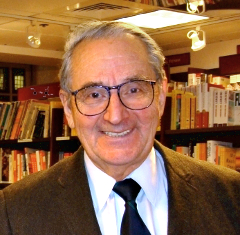
\includegraphics[width=\linewidth]{images/book3/corey.jpg}
\end{minipage}\hfill
\begin{minipage}[t]{0.76\linewidth}
\vspace{0pt}
Kimiawan selalu bernalar mundur dari target-target mereka, tetapi Elias
James Corey, sejak 1960-an, mengubah kebiasaan itu menjadi aturan-aturan
eksplisit: \omterm{def:b2:retrosynthesis:disconnection}{pemutusan}, \omterm{def:b2:retrosynthesis:disconnection}{sinton}, panah retrosintetik, dan bahkan program
komputer yang menerapkannya. Ia menerima Hadiah Nobel Kimia 1990 untuk teori
dan metodologi sintesis organik. (Foto: Trvthchem, CC0, Wikimedia Commons.)
\end{minipage}
\end{history}

\begin{safety}{\ghs[5mm]{GHS02}\,\ghs[5mm]{GHS03}\,\ghs[5mm]{GHS05}\,\ghs[5mm]{GHS06}\,\ghs[5mm]{GHS07}\,\ghs[5mm]{GHS08}}
Oksalil klorida bersifat korosif, beracun, dan bereaksi dengan air sambil
melepaskan hidrogen klorida; oksidasi Swern melepaskan karbon monoksida dan
dimetil sulfida yang berbau busuk, sehingga dijalankan di dalam lemari asam.
Periodinana Dess--Martin adalah pengoksidasi dan tidak boleh dipanaskan.
Pereaksi kromium(VI) kini dihindari bila ada alternatifnya.
% ledger: ghs:oxalyl-chloride, ghs:DMSO, ghs:DMP
\end{safety}

\section{Latihan}

\begin{exercise}[$\star$]\label{exo:b2:retrosynthesis:1}
Putuskan setiap alkohol menjadi senyawa karbonil dan pereaksi Grignard
(berikan setiap kemungkinan): 2-fenilpropan-2-ol, pentan-3-ol,
1-sikloheksiletanol, 2-metilbutan-2-ol, 1-feniletanol.
\end{exercise}

\begin{exercise}[$\star$]\label{exo:b2:retrosynthesis:2}
Untuk \omterm{def:b2:retrosynthesis:disconnection}{pemutusan} 1-feniletanol pada ikatan \ce{C-C}, sebutkan kedua
\omterm{def:b2:retrosynthesis:disconnection}{sintonnya}, nyatakan mana yang donor, dan berikan \omterm{def:b2:retrosynthesis:disconnection}{ekuivalen sintetik} untuk
masing-masing.
\end{exercise}

\begin{exercise}[$\star$]\label{exo:b2:retrosynthesis:3}
Sebuah jalur lima tahap mempunyai rendemen tahap 90, 85, 80, 95, dan 70~\%. Hitunglah rendemen keseluruhannya.
\end{exercise}

\begin{exercise}[$\star$]\label{exo:b2:retrosynthesis:4}
Etil 4-oksopentanoat harus diubah menjadi 5-hidroksipentan-2-on.
Rencanakan jalurnya dengan gugus pelindung, dan jelaskan mengapa gugus itu
diperlukan.
\end{exercise}

\begin{exercise}[$\star\star$]\label{exo:b2:retrosynthesis:5}
Usulkan retrosintesis butana-1,3-diol dari senyawa-senyawa dengan paling
banyak dua karbon, dengan satu FGI dan satu \omterm{def:b2:retrosynthesis:disconnection}{pemutusan} dua gugus.
\end{exercise}

\begin{exercise}[$\star\star$]\label{exo:b2:retrosynthesis:6}
Putuskan 1-(sikloheks-3-en-1-il)etan-1-on melalui \omterm{def:b2:frontier-orbitals:diels-alder}{reaksi Diels--Alder}.
\end{exercise}

\begin{exercise}[$\star\star$]\label{exo:b2:retrosynthesis:7}
Putuskan 4,4-dimetilsikloheks-2-en-1-on melalui \omterm{def:b2:conjugate-additions:robinson}{anulasi Robinson}.
\end{exercise}

\begin{exercise}[$\star\star$]\label{exo:b2:retrosynthesis:8}
1-Fenilbutan-1-on dapat dibuat dalam satu tahap melalui \omterm{def:b2:aromatic-substitution:friedel-crafts}{asilasi
Friedel--Crafts}, atau dalam dua tahap dari benzaldehida. Tuliskan kedua
jalur itu dan bandingkan.
\end{exercise}

\begin{exercise}[$\star\star$]\label{exo:b2:retrosynthesis:9}
Heksanal diinginkan dari heksan-1-ol. Pereaksi manakah yang
menghasilkannya, dan manakah yang justru akan menghasilkan asam heksanoat?
Jelaskan.
\end{exercise}

\begin{exercise}[$\star\star\star$]\label{exo:b2:retrosynthesis:10}
Dalam 4-aminobutan-1-ol, amina harus bereaksi lebih dahulu dengan \omterm{def:b2:acyl-substitution:derivative}{asil
klorida} dalam satu tahap, dan alkohol belakangan dengan \omterm{def:b2:acyl-substitution:derivative}{asil klorida} lain.
Usulkan sepasang \omterm{def:b2:retrosynthesis:orthogonal}{gugus pelindung ortogonal} dan urutannya.
\end{exercise}

\begin{exercise}[$\star\star\star$]\label{exo:b2:retrosynthesis:11}
Usulkan sintesis heksana-2,5-dion, sebuah senyawa 1,4-dikarbonil, dari etil 3-oksobutanoat.
\end{exercise}

\begin{exercise}[$\star\star\star$]\label{exo:b2:retrosynthesis:12}
6-Metilhept-5-en-2-on, \ce{(CH3)2C=CHCH2CH2COCH3}, adalah zat antara
pewangi. Usulkan rencana lengkap dari etil 3-oksobutanoat dan sebuah halida:
retrosintesis, jalur maju, dan tahap yang melepaskan esternya.
\end{exercise}

\section{Soal: Keton Rasberi}

\begin{problem}[{Soal akhir pekan --- retrosintesis sebuah senyawa perisa,
fenol dan perlu tidaknya fenol itu dilindungi, alternatif dengan paladium,
dan penilaian jalur-jalurnya}]
\label{pb:b2:retrosynthesis:1}
Keton rasberi, 4-(4-hidroksifenil)butan-2-on, ditemukan dalam buah rasberi
dan buah-buahan lain dan dipakai sebagai perisa dan dalam industri
wewangian. Data latihan: rendemen tahap jalur \omterm{def:b2:enolates-aldol:aldol}{aldol}, 85~\% (kondensasi)
dan 92~\% (hidrogenasi). Massa molar (\unit{g/mol}): C 12.011, H 1.008, O 15.999, N 14.007,
I 126.90. $\mathrm pK_a$ fenol adalah 9.99.
% ledger: use:raspberry-ketone, aw:C, aw:H, aw:O, aw:N, aw:I, pka:phenol, ghs:raspberry-ketone, ghs:4-iodophenol, ghs:MVK

\medskip
\noindent\textbf{Bagian I --- Retrosintesis.}
\begin{enumerate}
  \item Gambarlah targetnya dan sebutkan gugus-gugus fungsinya.
  \item FGI manakah yang mengubah satuan \ce{ArCH2CH2CO} menjadi pola dengan
        \omterm{def:b2:retrosynthesis:disconnection}{pemutusan} yang dikenal?
  \item Tuliskan keton tak jenuh yang diperoleh, beserta geometrinya.
  \item Pola dua gugus apakah yang dikandungnya, dan reaksi apakah yang membuatnya?
  \item Sebutkan kedua bahan awalnya.
  \item Mengapa \omterm{def:b2:enolates-aldol:aldol}{aldol} silang ini menghasilkan satu produk utama?
  \item Tuliskan jalur majunya dalam dua tahap, beserta kondisinya.
\end{enumerate}

\medskip
\noindent\textbf{Bagian II --- Fenol.}
\begin{enumerate}[resume]
  \item Dalam natrium hidroksida berair, dalam bentuk apakah
        4-hidroksibenzaldehida berada? Gunakan
        $\mathrm pK_a$.
  \item Bagaimana bentuk itu mengubah keelektrofilikan aldehidanya?
  \item Seandainya fenol itu dilindungi, gugus manakah yang akan dilepaskan
        oleh tahap kedua tanpa biaya tambahan? Jelaskan.
  \item Hitunglah tahap-tahap jalur dengan perlindungan itu.
  \item Apakah cincin benzena terancam dalam hidrogenasi?
  \item Dilindungi atau tidak? Simpulkan.
\end{enumerate}

\medskip
\noindent\textbf{Bagian III --- Alternatif dengan paladium.}
\begin{enumerate}[resume]
  \item Putuskan keton tak jenuh itu pada ikatan antara cincin dan rantai:
        pasangan Heck yang mana?
  \item Tuliskan reaksi Heck dengan trietilamina sebagai basa.
  \item Pada karbon but-3-en-2-on manakah gugus aril berakhir, dan mengapa?
  \item Sebutkan tahap-tahap \omterm{def:b2:catalytic-cycles:cycle}{siklus katalitiknya}.
  \item Hitunglah ekonomi atom tahap Heck, dengan memperhitungkan trietilamina.
  \item Hitunglah ekonomi atom \omterm{def:b2:enolates-aldol:aldol}{kondensasi aldol}.
\end{enumerate}

\medskip
\noindent\textbf{Bagian IV --- Menilai jalur-jalur.}
\begin{enumerate}[resume]
  \item Berapakah ekonomi atom hidrogenasinya?
  \item Hitunglah ekonomi atom keseluruhan jalur \omterm{def:b2:enolates-aldol:aldol}{aldol}.
  \item Ikatan rangkap manakah yang direduksi oleh hidrogenasi, dan mengapa ketonnya bertahan?
  \item Bandingkan pereaksi kedua jalur dari segi biaya dan bahaya.
  \item Jalur manakah yang akan dipilih?
  \item Apa pengaruh tahap ketiga dengan rendemen 90~\% terhadap rendemen keseluruhan?
  \item Nyatakan rendemen keseluruhan jalur \omterm{def:b2:enolates-aldol:aldol}{aldol} dua tahap.
\end{enumerate}
\end{problem}
